\documentclass[border=18pt]{standalone}
\usepackage[T1]{fontenc}
\usepackage[utf8]{inputenc}
\usepackage{circuitikz}
\usepackage{amsmath,amssymb}
\usetikzlibrary{positioning,calc}
\ctikzset{bipoles/length=1.15cm, font=\small}

\definecolor{tinta}{HTML}{1E293B}
\definecolor{ambar}{HTML}{C2410C}
\definecolor{azul}{HTML}{0E7490}
\definecolor{verde}{HTML}{15803D}
\definecolor{rojo}{HTML}{B91C1C}
\definecolor{gris}{HTML}{6B7280}
\definecolor{panel}{HTML}{F1F5F9}

\begin{document}
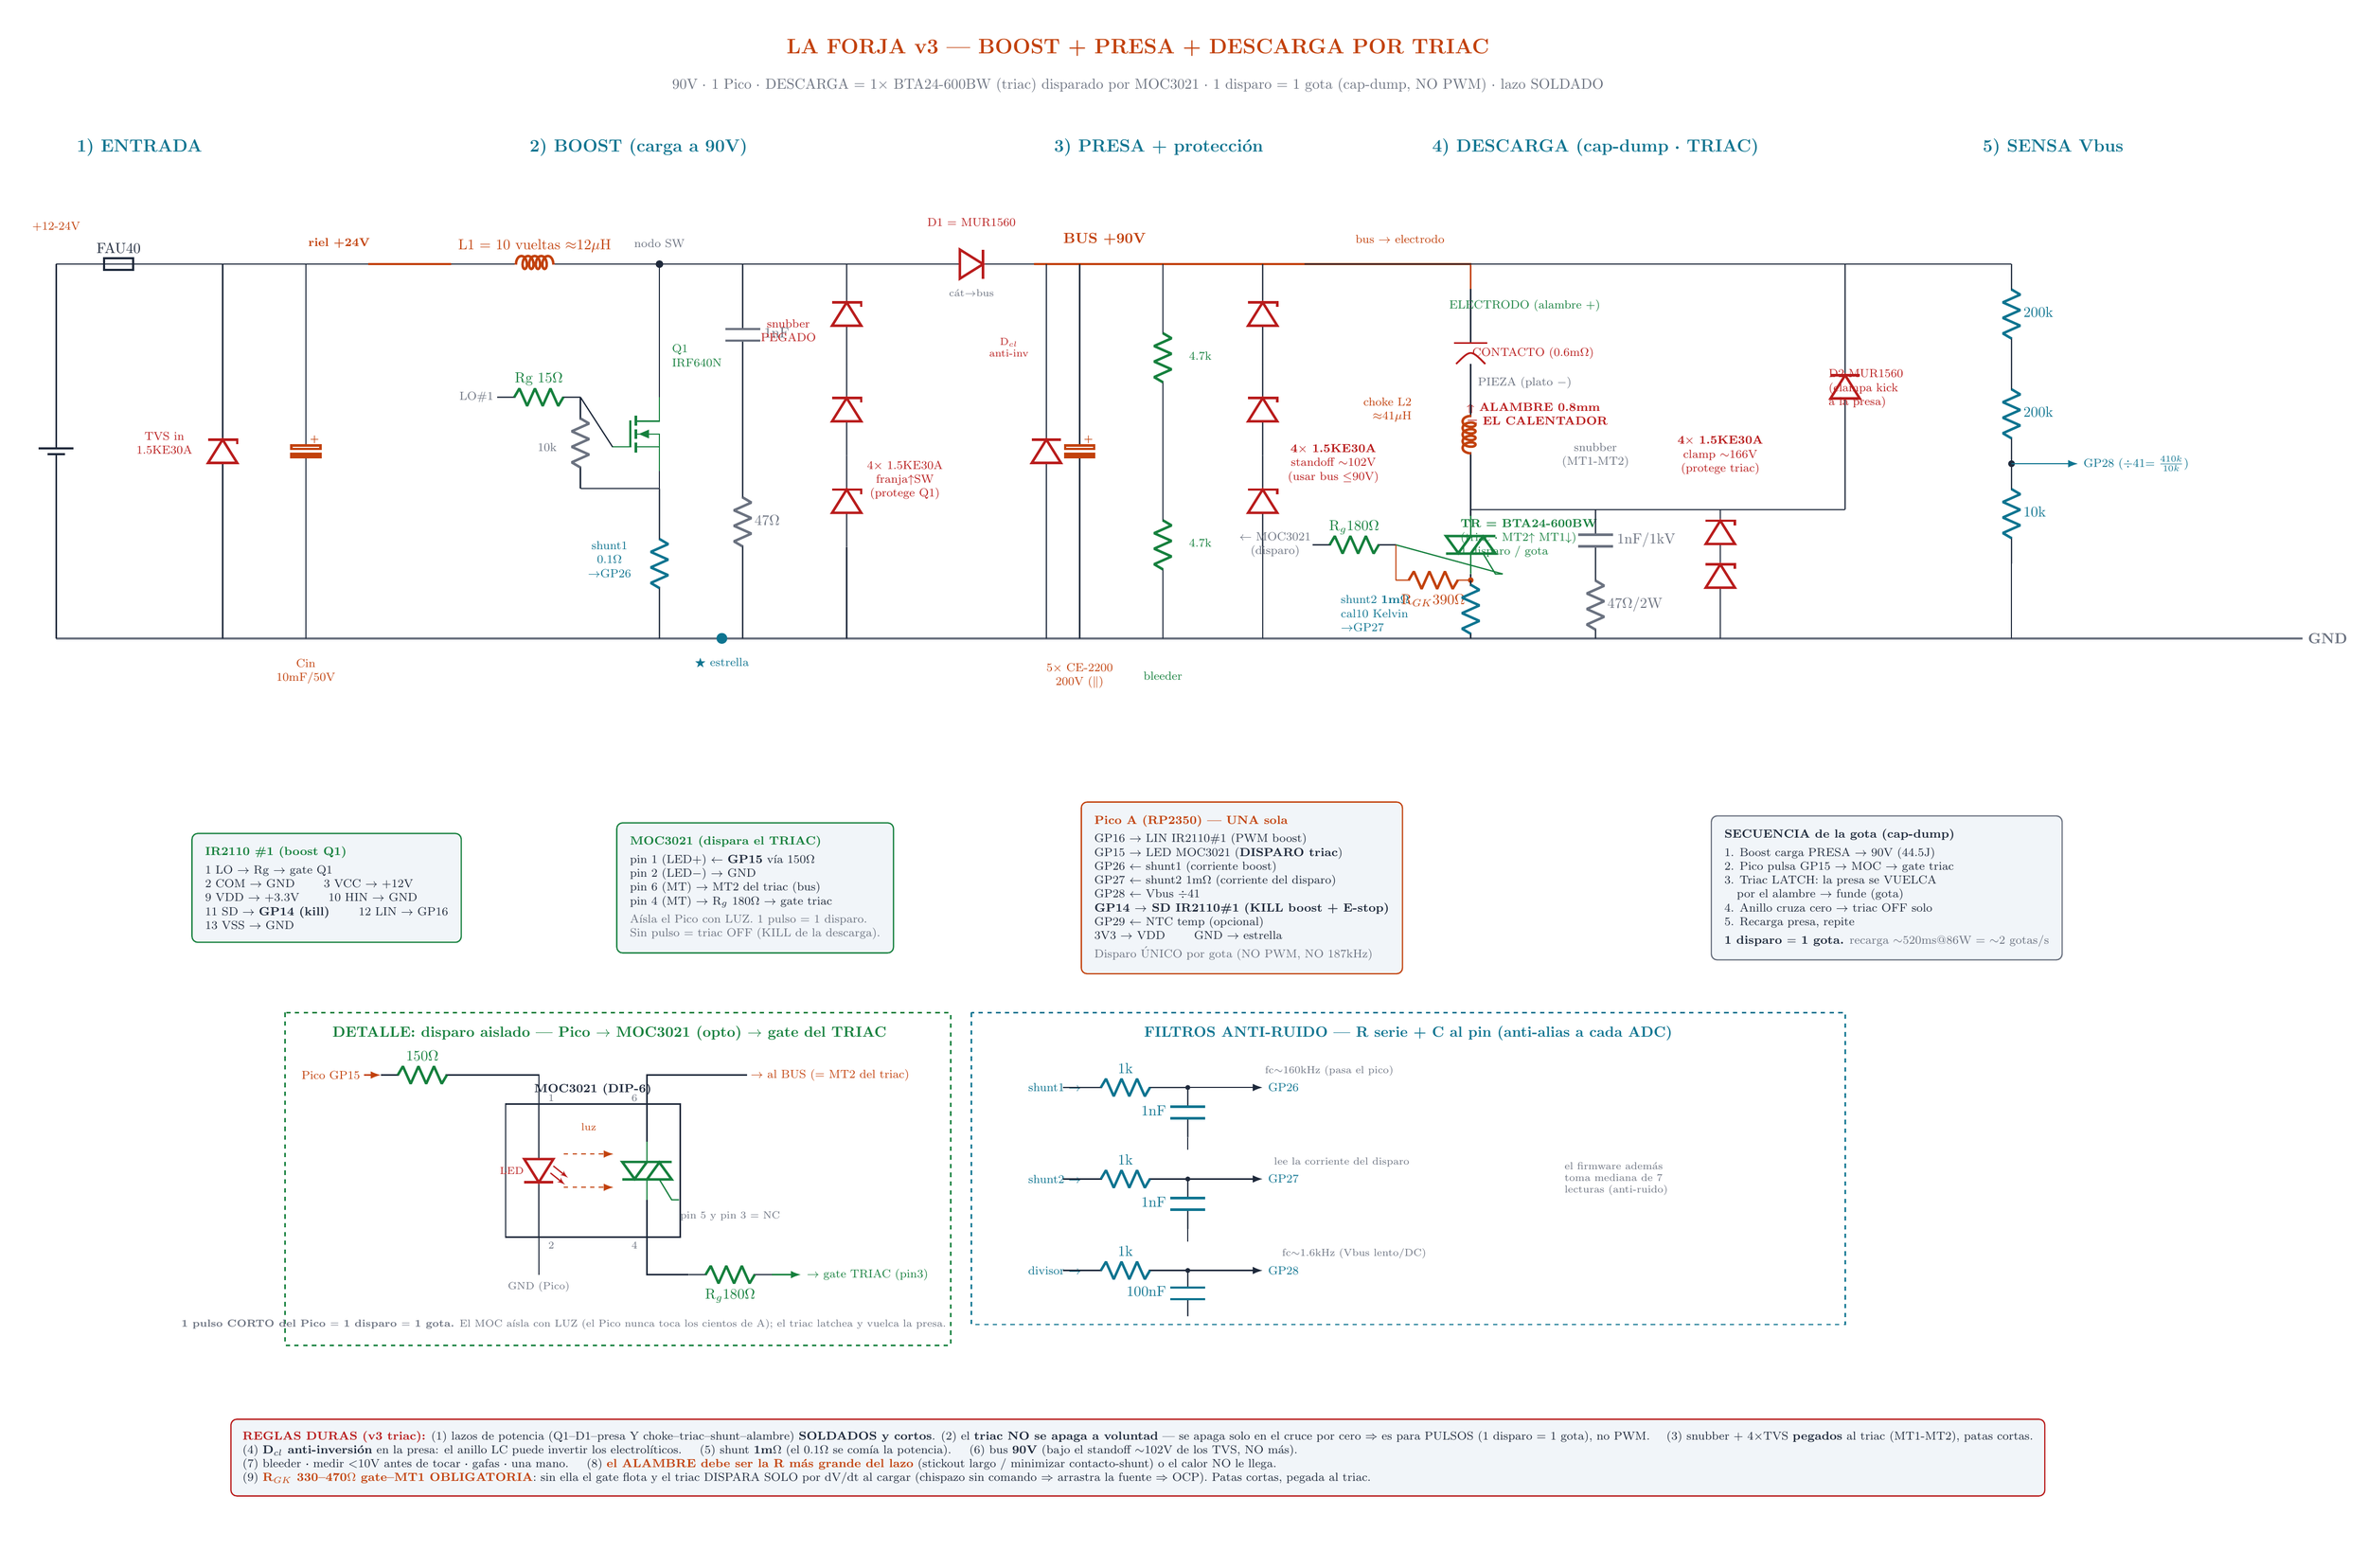
\begin{tikzpicture}[color=tinta, every node/.style={text=tinta}, line width=0.85pt]
\fill[white] (-11,-31) rectangle (45,6);

% ===== TITULO =====
\node[text=ambar, font=\bfseries\Large] at (16,5.2) {LA FORJA v3 — BOOST + PRESA + DESCARGA POR TRIAC};
\node[text=gris, font=\normalsize] at (16,4.3) {90V · 1 Pico · DESCARGA = 1$\times$ BTA24-600BW (triac) disparado por MOC3021 · 1 disparo = 1 gota (cap-dump, NO PWM) · lazo SOLDADO};

% ===== RIEL GND =====
\draw[gris, line width=1.4pt] (-10,-9) -- (44,-9);
\node[text=gris, font=\bfseries] at (44.6,-9){GND};
\fill[azul] (6,-9) circle (0.13); \node[text=azul, font=\footnotesize] at (6,-9.6){$\bigstar$ estrella};

% ========================= 1) ENTRADA =========================
\node[text=azul, font=\bfseries\large] at (-8,2.8){1) ENTRADA};
\draw (-10,0) to[battery1] (-10,-9);
\node[text=ambar, font=\footnotesize, align=center] at (-10,0.9){+12-24V};
\draw (-10,0) to[fuse, l=\textcolor{tinta}{FAU40}] (-7,0);
\draw (-7,0) -- (-2.5,0);
\draw (-6,0) to[empty Zener diode, invert, color=rojo] (-6,-9);
\node[text=rojo, font=\footnotesize, align=center] at (-7.4,-4.3){TVS in\\1.5KE30A};
\draw (-4,0) to[ecapacitor, color=ambar] (-4,-9);
\node[text=ambar, font=\footnotesize, align=center] at (-4,-9.8){Cin\\10mF/50V};
\draw[ambar, line width=1.2pt] (-2.5,0) -- (-0.5,0);
\node[text=ambar, font=\bfseries\footnotesize] at (-3.2,0.5){riel +24V};

% ========================= 2) BOOST (igual que v2) =========================
\node[text=azul, font=\bfseries\large] at (4,2.8){2) BOOST (carga a 90V)};
\draw (-0.5,0) to[L, l=\textcolor{ambar}{L1 = 10 vueltas $\approx$12$\mu$H}, color=ambar] (3.5,0);
\draw (3.5,0) -- (10.5,0); \fill[tinta] (4.5,0) circle (0.09);
\node[font=\footnotesize, text=gris] at (4.5,0.5){nodo SW};
% Q1 low-side
\node[nigfete, anchor=D, color=verde, scale=1.15] (Q1) at (4.5,-3.2){};
\draw (4.5,0) -- (Q1.D);
\node[text=verde, font=\footnotesize, align=left] at (5.4,-2.2){Q1\\IRF640N};
\draw (Q1.G) -- (2.6,-3.2);
\draw (2.6,-3.2) to[R, l_=\textcolor{verde}{Rg 15$\Omega$}, color=verde] (0.6,-3.2);
\node[font=\footnotesize, text=gris] at (0.1,-3.2){LO\#1};
\draw (2.6,-3.2) to[R, color=gris] (2.6,-5.4); \node[text=gris,font=\footnotesize] at (1.8,-4.4){10k};
\draw (2.6,-5.4) -- (4.5,-5.4);
\draw (Q1.S) -- (4.5,-5.4);
\draw (4.5,-5.4) to[R, color=azul] (4.5,-9);
\node[text=azul, font=\footnotesize, align=center] at (3.3,-7.1){shunt1\\0.1$\Omega$\\$\to$GP26};
% snubber Q1
\draw (6.5,0) to[C, l=\textcolor{gris}{1nF}, color=gris] (6.5,-3.4);
\draw (6.5,-3.4) to[R, l=\textcolor{gris}{47$\Omega$}, color=gris] (6.5,-9);
\node[text=rojo, font=\footnotesize, align=center] at (7.6,-1.6){snubber\\PEGADO};
% 4x TVS drain Q1
\draw (9,0) to[empty Zener diode, invert, color=rojo] (9,-2.4);
\draw (9,-2.4) to[empty Zener diode, invert, color=rojo] (9,-4.6);
\draw (9,-4.6) to[empty Zener diode, invert, color=rojo] (9,-6.8);
\draw (9,-6.8) -- (9,-9);
\node[text=rojo, font=\footnotesize, align=center] at (10.4,-5.2){4$\times$ 1.5KE30A\\franja$\uparrow$SW\\(protege Q1)};
% D1 al bus
\draw (10.5,0) to[D, color=rojo] (13.5,0);
\node[text=rojo, font=\footnotesize] at (12,1.0){D1 = MUR1560};
\node[text=gris,font=\scriptsize] at (12,-0.7){cát$\to$bus};

% ========================= 3) PRESA =========================
\node[text=azul, font=\bfseries\large] at (16.5,2.8){3) PRESA + protección};
\draw[ambar, line width=1.2pt] (13.5,0) -- (20,0);
\node[text=ambar, font=\bfseries] at (15.2,0.6){BUS +90V};
% D clamp anti-inversion (NUEVO para triac)
\draw (13.8,0) to[D, color=rojo, invert] (13.8,-9);
\node[text=rojo, font=\scriptsize, align=center] at (12.9,-2.0){D$_{cl}$\\anti-inv};
\draw (14.6,0) to[ecapacitor, color=ambar] (14.6,-9);
\node[text=ambar, font=\footnotesize, align=center] at (14.6,-9.9){5$\times$ CE-2200\\200V ($\parallel$)};
\draw (16.6,0) to[R, color=verde] (16.6,-4.5);
\draw (16.6,-4.5) to[R, color=verde] (16.6,-9);
\node[text=verde, font=\footnotesize] at (17.5,-2.2){4.7k}; \node[text=verde, font=\footnotesize] at (17.5,-6.7){4.7k};
\node[text=verde, font=\footnotesize] at (16.6,-9.9){bleeder};
% TVS DEL BUS
\draw (19,0) to[empty Zener diode, invert, color=rojo] (19,-2.4);
\draw (19,-2.4) to[empty Zener diode, invert, color=rojo] (19,-4.6);
\draw (19,-4.6) to[empty Zener diode, invert, color=rojo] (19,-6.8);
\draw (19,-6.8) -- (19,-9);
\node[text=rojo, font=\footnotesize, align=center] at (20.7,-4.8){\textbf{4$\times$ 1.5KE30A}\\standoff $\sim$102V\\(usar bus $\le$90V)};

% ========================= 4) DESCARGA (cap-dump por TRIAC) =========================
\node[text=azul, font=\bfseries\large] at (27,2.8){4) DESCARGA (cap-dump · TRIAC)};
\draw[ambar, line width=1.2pt] (20,0) -- (24,0) -- (24,-0.6);
\node[text=ambar, font=\footnotesize] at (22.3,0.6){bus $\to$ electrodo};
% electrodo
\draw (24,-0.6) -- (24,-1.4);
\node[text=verde, font=\footnotesize, align=left] at (25.3,-1.0){ELECTRODO (alambre +)};
% contacto / junta
\draw (24,-1.4) -- (24,-1.9);
\draw[rojo, line width=1.2pt] (23.6,-1.9) -- (24.4,-1.9);
\draw[rojo, line width=1.2pt] (23.65,-2.4) .. controls (24,-2.05) .. (24.35,-2.4);
\node[text=rojo, font=\footnotesize, align=left] at (25.5,-2.15){CONTACTO (0.6m$\Omega$)};
\draw (24,-2.4) -- (24,-2.9);
\node[text=gris, font=\footnotesize, align=left] at (25.3,-2.85){PIEZA (plato $-$)};
\node[text=rojo, font=\footnotesize, align=left] at (25.6,-3.6){\textbf{$\Uparrow$ ALAMBRE 0.8mm}\\\textbf{= EL CALENTADOR}};
% choke en el retorno
\draw (24,-2.9) to[L, color=ambar, mirror] (24,-5.3);
\node[text=ambar, font=\footnotesize, align=right] at (22.0,-3.5){choke L2\\$\approx$41$\mu$H};
% TRIAC (reemplaza al MOSFET Q2)
\draw (24,-5.3) -- (24,-5.9);
\draw (24,-5.9) to[triac, name=TR, color=verde] (24,-7.6);
\node[text=verde, font=\footnotesize, align=left] at (25.4,-6.6){\textbf{TR = BTA24-600BW}\\(triac · MT2$\uparrow$ MT1$\downarrow$)\\1 disparo / gota};
% gate del triac <- MOC3021
\draw[verde] (TR.gate) -- (22.2,-6.75);
\draw (22.2,-6.75) to[R, l_=\textcolor{verde}{R$_g$180$\Omega$}, color=verde] (20.2,-6.75);
\node[font=\footnotesize, text=gris, align=center] at (19.3,-6.75){$\leftarrow$ MOC3021\\(disparo)};
% *** R gate->MT1 (R_GK): mata el disparo espurio por dV/dt -- EL FIX (v3.1) ***
\draw[ambar, line width=0.9pt] (22.2,-6.75) -- (22.2,-7.6);
\draw[ambar] (22.2,-7.6) to[R, l_=\textcolor{ambar}{R$_{GK}$390$\Omega$}, color=ambar] (24,-7.6);
\fill[ambar] (24,-7.6) circle (0.07);
% shunt 1mOhm Kelvin (reemplaza 0.1ohm)
\draw (24,-7.6) to[R, color=azul] (24,-9);
\node[text=azul, font=\footnotesize, align=left] at (21.7,-8.4){shunt2 \textbf{1m$\Omega$}\\cal10 Kelvin\\$\to$GP27};
% nodo MT2 del triac (tap horizontal a la derecha)
\draw (24,-5.9) -- (33,-5.9);
% snubber del triac
\draw (27,-5.9) to[C, l=\textcolor{gris}{1nF/1kV}, color=gris] (27,-7.4);
\draw (27,-7.4) to[R, l=\textcolor{gris}{47$\Omega$/2W}, color=gris] (27,-9);
\node[text=gris, font=\footnotesize, align=center] at (27,-4.6){snubber\\(MT1-MT2)};
% 4x TVS del triac
\draw (30,-5.9) to[empty Zener diode, invert, color=rojo] (30,-7.0);
\draw (30,-7.0) to[empty Zener diode, invert, color=rojo] (30,-8.0);
\draw (30,-8.0) -- (30,-9);
\node[text=rojo, font=\footnotesize, align=center] at (30,-4.6){\textbf{4$\times$ 1.5KE30A}\\clamp $\sim$166V\\(protege triac)};
% D2: MT2 -> BUS (clampa el kick inductivo)
\draw (33,-5.9) to[D, color=rojo] (33,0);
\node[text=rojo, font=\footnotesize, align=left] at (33.5,-3.0){D2 MUR1560\\(clampa kick\\a la presa)};

% ========================= 5) SENSADO =========================
\node[text=azul, font=\bfseries\large] at (38,2.8){5) SENSA Vbus};
\draw (20,0) -- (37,0);
\draw (37,0) to[R, l=\textcolor{azul}{200k}, color=azul] (37,-2.4);
\draw (37,-2.4) to[R, l=\textcolor{azul}{200k}, color=azul] (37,-4.8);
\draw (37,-4.8) to[R, l=\textcolor{azul}{10k}, color=azul] (37,-7.2);
\draw (37,-7.2) -- (37,-9);
\fill[tinta] (37,-4.8) circle (0.08);
\draw[azul,-{Latex}] (37,-4.8) -- (38.6,-4.8) node[right,text=azul,font=\footnotesize]{GP28 ($\div$41$=\frac{410k}{10k}$)};

% ===================== CONTROL: IR2110 (boost) + MOC3021 (triac) + PICO =====================
\node[draw=verde, fill=panel, rounded corners, align=left, inner sep=9pt, font=\footnotesize] at (-3.5,-15)
 {\textbf{\textcolor{verde}{IR2110 \#1 (boost Q1)}}\\[3pt]
  1 LO $\to$ Rg $\to$ gate Q1\\
  2 COM $\to$ GND \qquad 3 VCC $\to$ +12V\\
  9 VDD $\to$ +3.3V \qquad 10 HIN $\to$ GND\\
  11 SD $\to$ \textbf{GP14 (kill)} \qquad 12 LIN $\to$ GP16\\
  13 VSS $\to$ GND};
\node[draw=verde, fill=panel, rounded corners, align=left, inner sep=9pt, font=\footnotesize] at (6.8,-15)
 {\textbf{\textcolor{verde}{MOC3021 (dispara el TRIAC)}}\\[3pt]
  pin 1 (LED+) $\leftarrow$ \textbf{GP15} vía 150$\Omega$\\
  pin 2 (LED$-$) $\to$ GND\\
  pin 6 (MT) $\to$ MT2 del triac (bus)\\
  pin 4 (MT) $\to$ R$_g$ 180$\Omega$ $\to$ gate triac\\[3pt]
  \textcolor{gris}{Aísla el Pico con LUZ. 1 pulso = 1 disparo.}\\
  \textcolor{gris}{Sin pulso $=$ triac OFF (KILL de la descarga).}};
\node[draw=ambar, fill=panel, rounded corners, align=left, inner sep=9pt, font=\footnotesize] at (18.5,-15)
 {\textbf{\textcolor{ambar}{Pico A (RP2350) — UNA sola}}\\[3pt]
  GP16 $\to$ LIN IR2110\#1 (PWM boost)\\
  GP15 $\to$ LED MOC3021 (\textbf{DISPARO triac})\\
  GP26 $\leftarrow$ shunt1 (corriente boost)\\
  GP27 $\leftarrow$ shunt2 1m$\Omega$ (corriente del disparo)\\
  GP28 $\leftarrow$ Vbus $\div$41\\
  \textbf{GP14 $\to$ SD IR2110\#1 (KILL boost + E-stop)}\\
  GP29 $\leftarrow$ NTC temp (opcional)\\
  3V3 $\to$ VDD \qquad GND $\to$ estrella\\[3pt]
  \textcolor{gris}{Disparo ÚNICO por gota (NO PWM, NO 187kHz)}};
\node[draw=gris, fill=panel, rounded corners, align=left, inner sep=9pt, font=\footnotesize] at (34,-15)
 {\textbf{SECUENCIA de la gota (cap-dump)}\\[3pt]
  1. Boost carga PRESA $\to$ 90V (44.5J)\\
  2. Pico pulsa GP15 $\to$ MOC $\to$ gate triac\\
  3. Triac LATCH: la presa se VUELCA\\
  \quad por el alambre $\to$ funde (gota)\\
  4. Anillo cruza cero $\to$ triac OFF solo\\
  5. Recarga presa, repite\\[3pt]
  \textbf{1 disparo $=$ 1 gota.} \textcolor{gris}{recarga $\sim$520ms@86W $=$ $\sim$2 gotas/s}};

\node[draw=rojo, fill=panel, rounded corners, align=left, inner sep=8pt, font=\footnotesize, text=tinta] at (16,-28.7)
 {\textcolor{rojo}{\textbf{REGLAS DURAS (v3 triac):}} (1) lazos de potencia (Q1--D1--presa Y choke--triac--shunt--alambre) \textbf{SOLDADOS y cortos}.
  (2) el \textbf{triac NO se apaga a voluntad} — se apaga solo en el cruce por cero $\Rightarrow$ es para PULSOS (1 disparo = 1 gota), no PWM. \quad (3) snubber + 4$\times$TVS \textbf{pegados} al triac (MT1-MT2), patas cortas.\\
  (4) \textbf{D$_{cl}$ anti-inversión} en la presa: el anillo LC puede invertir los electrolíticos. \quad (5) shunt \textbf{1m$\Omega$} (el 0.1$\Omega$ se comía la potencia). \quad (6) bus \textbf{90V} (bajo el standoff $\sim$102V de los TVS, NO más).\\
  (7) bleeder · medir $<$10V antes de tocar · gafas · una mano. \quad (8) \textcolor{ambar}{\textbf{el ALAMBRE debe ser la R más grande del lazo}} (stickout largo / minimizar contacto-shunt) o el calor NO le llega.\\
  (9) \textcolor{ambar}{\textbf{R$_{GK}$ 330--470$\Omega$ gate--MT1 OBLIGATORIA}}: sin ella el gate flota y el triac DISPARA SOLO por dV/dt al cargar (chispazo sin comando $\Rightarrow$ arrastra la fuente $\Rightarrow$ OCP). Patas cortas, pegada al triac.};

% ===================== DETALLE: disparo aislado Pico -> MOC3021 (opto) -> triac =====================
\draw[verde, dashed, line width=1pt] (-4.5,-18.0) rectangle (11.5,-26.0);
\node[text=verde, font=\bfseries] at (3.3,-18.5){DETALLE: disparo aislado — Pico $\to$ MOC3021 (opto) $\to$ gate del TRIAC};
% --- el MOC3021 dibujado REAL: LED + foto-triac acoplados por LUZ (DIP-6) ---
\draw[tinta, line width=0.9pt] (0.8,-20.2) rectangle (5.0,-23.4);
\node[text=tinta, font=\footnotesize\bfseries] at (2.9,-19.85){MOC3021 (DIP-6)};
% LED de entrada (anodo arriba=pin1, catodo abajo=pin2)
\draw (1.6,-20.2) to[leD, color=rojo] (1.6,-23.4);
\node[text=rojo, font=\scriptsize] at (0.95,-21.8){LED};
% foto-triac de salida (pin6 arriba, pin4 abajo); lo dispara la LUZ
\draw (4.2,-20.2) to[triac, name=PT, color=verde] (4.2,-23.4);
% acoplamiento optico (la luz dispara el foto-triac)
\draw[ambar, dashed, -{Latex}] (2.2,-21.4) -- (3.4,-21.4);
\draw[ambar, dashed, -{Latex}] (2.2,-22.2) -- (3.4,-22.2);
\node[text=ambar, font=\scriptsize] at (2.8,-20.75){luz};
% numeros de pin
\node[font=\scriptsize, text=gris] at (1.9,-20.05){1}; \node[font=\scriptsize, text=gris] at (1.9,-23.6){2};
\node[font=\scriptsize, text=gris] at (3.9,-20.05){6}; \node[font=\scriptsize, text=gris] at (3.9,-23.6){4};
\node[font=\scriptsize, text=gris, align=left] at (6.2,-22.9){pin 5 y pin 3 = NC};
% --- INPUT: GP15 -> 150ohm -> pin1(anodo) ; pin2(catodo) -> GND ---
\node[text=ambar, font=\footnotesize] at (-3.4,-19.5){Pico GP15};
\draw[ambar,-{Latex}] (-2.6,-19.5) -- (-2.2,-19.5);
\draw (-2.2,-19.5) to[R, l=\textcolor{verde}{150$\Omega$}, color=verde] (-0.2,-19.5);
\draw (-0.2,-19.5) -- (1.6,-19.5) -- (1.6,-20.2);
\draw (1.6,-23.4) -- (1.6,-24.3); \node[text=gris,font=\scriptsize] at (1.6,-24.6){GND (Pico)};
% --- OUTPUT: pin6 -> BUS(MT2) ; pin4 -> Rg180 -> gate del triac ---
\draw (4.2,-20.2) -- (4.2,-19.5) -- (6.6,-19.5);
\node[text=ambar, font=\footnotesize, align=left] at (8.6,-19.5){$\to$ al BUS (= MT2 del triac)};
\draw (4.2,-23.4) -- (4.2,-24.3) -- (5.2,-24.3);
\draw (5.2,-24.3) to[R, l_=\textcolor{verde}{R$_g$180$\Omega$}, color=verde] (7.2,-24.3);
\draw[verde,-{Latex}] (7.2,-24.3) -- (7.9,-24.3);
\node[text=verde, font=\footnotesize, align=left] at (9.5,-24.3){$\to$ gate TRIAC (pin3)};
% nota
\node[text=gris, font=\scriptsize, align=left] at (2.2,-25.5){\textbf{1 pulso CORTO del Pico $=$ 1 disparo $=$ 1 gota.} El MOC aísla con LUZ (el Pico nunca toca los cientos de A); el triac latchea y vuelca la presa.};

% ===================== FILTROS ANTI-RUIDO (RC a cada ADC) =====================
\draw[azul, dashed, line width=1pt] (12,-18.0) rectangle (33,-25.5);
\node[text=azul, font=\bfseries] at (22.5,-18.5){FILTROS ANTI-RUIDO — R serie + C al pin (anti-alias a cada ADC)};
% fila GP26
\node[text=azul, font=\footnotesize, align=right] at (14,-19.8){shunt1 $\to$};
\draw (14.2,-19.8) to[R, l=\textcolor{azul}{1k}, color=azul] (17.2,-19.8); \fill[tinta](17.2,-19.8)circle(0.06);
\draw[-{Latex}] (17.2,-19.8)--(19,-19.8) node[right,text=azul,font=\footnotesize]{GP26};
\draw (17.2,-19.8) to[C, l_=\textcolor{azul}{1nF}, color=azul] (17.2,-21.0); \draw(17.2,-21.0)--(17.2,-21.3);
\node[text=gris,font=\scriptsize] at (20.6,-19.4){fc$\sim$160kHz (pasa el pico)};
% fila GP27
\node[text=azul, font=\footnotesize, align=right] at (14,-22.0){shunt2 $\to$};
\draw (14.2,-22.0) to[R, l=\textcolor{azul}{1k}, color=azul] (17.2,-22.0); \fill[tinta](17.2,-22.0)circle(0.06);
\draw[-{Latex}] (17.2,-22.0)--(19,-22.0) node[right,text=azul,font=\footnotesize]{GP27};
\draw (17.2,-22.0) to[C, l_=\textcolor{azul}{1nF}, color=azul] (17.2,-23.2); \draw(17.2,-23.2)--(17.2,-23.5);
\node[text=gris,font=\scriptsize] at (20.9,-21.6){lee la corriente del disparo};
% fila GP28
\node[text=azul, font=\footnotesize, align=right] at (14,-24.2){divisor $\to$};
\draw (14.2,-24.2) to[R, l=\textcolor{azul}{1k}, color=azul] (17.2,-24.2); \fill[tinta](17.2,-24.2)circle(0.06);
\draw[-{Latex}] (17.2,-24.2)--(19,-24.2) node[right,text=azul,font=\footnotesize]{GP28};
\draw (17.2,-24.2) to[C, l_=\textcolor{azul}{100nF}, color=azul] (17.2,-25.3);
\node[text=gris,font=\scriptsize] at (21.2,-23.8){fc$\sim$1.6kHz (Vbus lento/DC)};
\node[text=gris, font=\scriptsize, align=left] at (27.5,-22.0){el firmware además\\toma mediana de 7\\lecturas (anti-ruido)};

\end{tikzpicture}
\end{document}
